\documentclass{classes/report}

\usepackage{enumitem}
\pagestyle{empty}

\begin{document}
% textlint-disable ja-technical-writing/ja-no-mixed-period
基礎電子工学 \ 第12回 \ 課題
% textlint-enable ja-technical-writing/ja-no-mixed-period
\begin{flushright}
    \underline{\ 学籍番号 \ 2397002 \ 氏名 \ 杉本 謙仁 \ }
\end{flushright}

\bigskip

\begin{enumerate}
    \item 金属とp型半導体の接触の場合のショットキー接触,およびオーミック接触のエネルギーバンド図を描け.
\end{enumerate}

\begin{figure}[H]
    \centering
    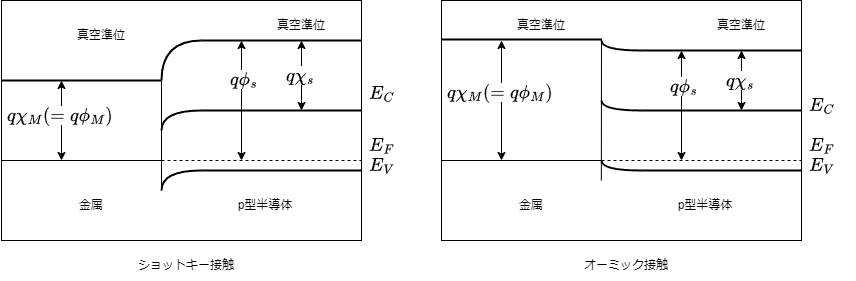
\includegraphics[width=1\linewidth]{figures/energyband.png}
    \caption{ショットキー接触とオーミック接触のエネルギーバンド図}
\end{figure}

\bigskip

\begin{enumerate}[resume]
    \item 金属とn型シリコン半導体を接触させ,$1.8 [\mathrm{V}]$の逆方向電圧を印加した.空乏層幅と空乏層容量を求めよ.ただし,シリコンの比誘電率を12,電子密度を$1017 [\mathrm{cm}^{-3}]$,接触面積を$0.2 [\mathrm{mm}^2]$,拡散電位を$0.4 [\mathrm{V}]$とする.
\end{enumerate}

\begin{equation}
    \begin{split}
        \omega & = \sqrt{\frac{2\epsilon_0 \epsilon_s}{qN_d}} \sqrt{V_d - V}                                                                   \\
               & = \sqrt{\frac{2 \times 8.854 \times 10^{-12} \times 12}{1.602 \times 10^{-19} \times 10^{17} \times 10^{6}}} \sqrt{0.4 + 1.8} \\
               & = 1.7 \times 10^{-7} [\mathrm{m}]                                                                                             \\
               & = 0.17 [\mathrm{\mu m}]                                                                                                       \\
        C      & = \frac{\epsilon}{\omega} \cdot S                                                                                             \\
               & = \frac{8.854 \times 10^{-12} \times 12}{1.7 \times 10^{-7}} \times 0.2 \times 10^{-6}                                        \\
               & = 1.2 \times 10^{-10}                                                                                                         \\
               & = 120 [\mathrm{pF}]
    \end{split}
\end{equation}

\end{document}